% **************************************************************************************************************
% A Classic Thesis Style
% An Homage to The Elements of Typographic Style
%
% Copyright (C) 2018 André Miede and Ivo Pletikosić
%
% If you like the style then I would appreciate a postcard. My address
% can be found in the file ClassicThesis.pdf. A collection of the
% postcards I received so far is available online at
% http://postcards.miede.de
%
% License:
% This program is free software; you can redistribute it and/or modify
% it under the terms of the GNU General Public License as published by
% the Free Software Foundation; either version 2 of the License, or
% (at your option) any later version.
%
% This program is distributed in the hope that it will be useful,
% but WITHOUT ANY WARRANTY; without even the implied warranty of
% MERCHANTABILITY or FITNESS FOR A PARTICULAR PURPOSE.  See the
% GNU General Public License for more details.
%
% You should have received a copy of the GNU General Public License
% along with this program; see the file COPYING.  If not, write to
% the Free Software Foundation, Inc., 59 Temple Place - Suite 330,
% Boston, MA 02111-1307, USA.
%
% PLEASE SEE ALSO THE AUTHORS' NOTE REGARDING THIS LICENSE
% IN THE DOCUMENTATION (ClassicThesis.pdf --> Chapter 1 / Chapter01.tex)
% **************************************************************************************************************
\RequirePackage{silence} % :-\
    \WarningFilter{scrreprt}{Usage of package `titlesec'}
    %\WarningFilter{scrreprt}{Activating an ugly workaround}
    \WarningFilter{titlesec}{Non standard sectioning command detected}
\documentclass[ twoside,openright,titlepage,numbers=noenddot,%1headlines,
                headinclude,footinclude,cleardoublepage=empty,abstract=on,
                BCOR=5mm,paper=a4,fontsize=11pt
                ]{scrreprt}

%********************************************************************
% Note: Make all your adjustments in here
%*******************************************************
% LTex: enabled=false
% ****************************************************************************************************
% classicthesis-config.tex
% formerly known as loadpackages.sty, classicthesis-ldpkg.sty, and classicthesis-preamble.sty
% Use it at the beginning of your ClassicThesis.tex, or as a LaTeX Preamble
% in your ClassicThesis.{tex,lyx} with \input{classicthesis-config}
% ****************************************************************************************************
% If you like the classicthesis, then I would appreciate a postcard.
% My address can be found in the file ClassicThesis.pdf. A collection
% of the postcards I received so far is available online at
% http://postcards.miede.de
% ****************************************************************************************************


% ****************************************************************************************************
% 0. Set the encoding of your files. UTF-8 is the only sensible encoding nowadays. If you can't read
% äöüßáéçèê∂åëæƒÏ€ then change the encoding setting in your editor, not the line below. If your editor
% does not support utf8 use another editor!
% ****************************************************************************************************
\PassOptionsToPackage{utf8}{inputenc}
\usepackage{inputenc}

\PassOptionsToPackage{T1}{fontenc} % T2A for cyrillics
\usepackage{fontenc}


% ****************************************************************************************************
% 1. Configure classicthesis for your needs here, e.g., remove "drafting" below
% in order to deactivate the time-stamp on the pages
% (see ClassicThesis.pdf for more information):
% ****************************************************************************************************
\PassOptionsToPackage{
  drafting=false,    % print version information on the bottom of the pages
  tocaligned=false, % the left column of the toc will be aligned (no indentation)
  dottedtoc=true,  % page numbers in ToC flushed right
  eulerchapternumbers=true, % use AMS Euler for chapter font (otherwise Palatino)
  linedheaders=false,       % chaper headers will have line above and beneath
  floatperchapter=true,     % numbering per chapter for all floats (i.e., Figure 1.1)
  eulermath=false,  % use awesome Euler fonts for mathematical formulae (only with pdfLaTeX)
  beramono=true,    % toggle a nice monospaced font (w/ bold)
  palatino=true,    % deactivate standard font for loading another one, see the last section at the end of this file for suggestions
  style=classicthesis % classicthesis, arsclassica
}{classicthesis}


% ****************************************************************************************************
% 2. Personal data and user ad-hoc commands (insert your own data here)
% ****************************************************************************************************
\newcommand{\myTitle}{Improving Primary Key Detection\linebreak[1] with Machine Learning\xspace}
\newcommand{\myTitleHyperref}{Improving Primary Key Detection with Machine Learning\xspace}
\newcommand{\mySubtitle}{\xspace}
\newcommand{\myDegree}{Bachelor Thesis\xspace}
\newcommand{\myName}{Janek Prange\xspace}
\newcommand{\myProf}{Prof. Dr. Ziawasch Abedjan\xspace}
\newcommand{\myOtherProf}{Prof. Dr. Sören Auer\xspace}
\newcommand{\mySupervisor}{Prof. Dr. Ziawasch Abedjan\xspace}
\newcommand{\myFaculty}{Fakultät für Elektrotechnik und Informatik\xspace}
\newcommand{\myDepartment}{Institut für Praktische Informatik\xspace}
\newcommand{\myUni}{Leibniz Universität Hannover\xspace}
\newcommand{\myLocation}{Hannover\xspace}
\newcommand{\myTime}{03.07.2022\xspace}
\newcommand{\myVersion}{\classicthesis}

% ********************************************************************
% Setup, finetuning, and useful commands
% ********************************************************************
\providecommand{\mLyX}{L\kern-.1667em\lower.25em\hbox{Y}\kern-.125emX\@}
\newcommand{\ie}{i.\,e.}
\newcommand{\Ie}{I.\,e.}
\newcommand{\eg}{e.\,g.}
\newcommand{\Eg}{E.\,g.}
% ****************************************************************************************************


% ****************************************************************************************************
% 3. Loading some handy packages
% ****************************************************************************************************
% ********************************************************************
% Packages with options that might require adjustments
% ********************************************************************
\PassOptionsToPackage{ngerman, american}{babel} % change this to your language(s), main language last
% Spanish languages need extra options in order to work with this template
%\PassOptionsToPackage{spanish,es-lcroman}{babel}
\usepackage{babel}

\usepackage{csquotes}
\PassOptionsToPackage{%
  %backend=biber,bibencoding=utf8, %instead of bibtex
  backend=bibtex8,bibencoding=ascii,%
  language=auto,%
  % style=numeric-comp,%
  %style=authoryear-comp, % Author 1999, 2010
  %bibstyle=authoryear,dashed=false, % dashed: substitute rep. author with ---
  sorting=nyt, % name, year, title
  maxbibnames=10, % default: 3, et al.
  %backref=true,%
  natbib=true % natbib compatibility mode (\citep and \citet still work)
}{biblatex}
\usepackage{biblatex}
\DeclareFieldFormat{url}{\newline\mkbibacro{URL}\addcolon\nobreakspace\url{#1}}

\PassOptionsToPackage{fleqn}{amsmath}       % math environments and more by the AMS
\usepackage{amsmath}

\usepackage[strict]{changepage} %Veränderungen an Textblöcken
\usepackage{bm}

% ********************************************************************
% General useful packages
% ********************************************************************
\usepackage{graphicx} %
\usepackage{scrhack} % fix warnings when using KOMA with listings package
\usepackage{xspace} % to get the spacing after macros right
\PassOptionsToPackage{printonlyused,smaller}{acronym}
\usepackage{acronym} % nice macros for handling all acronyms in the thesis
%\renewcommand{\bflabel}[1]{{#1}\hfill} % fix the list of acronyms --> no longer working
%\renewcommand*{\acsfont}[1]{\textsc{#1}}
%\renewcommand*{\aclabelfont}[1]{\acsfont{#1}}
%\def\bflabel#1{{#1\hfill}}
\def\bflabel#1{{\acsfont{#1}\hfill}}
\def\aclabelfont#1{\acsfont{#1}}
% ****************************************************************************************************
%\usepackage{pgfplots} % External TikZ/PGF support (thanks to Andreas Nautsch)
%\usetikzlibrary{external}
%\tikzexternalize[mode=list and make, prefix=ext-tikz/]
% ****************************************************************************************************


% ****************************************************************************************************
% 4. Setup floats: tables, (sub)figures, and captions
% ****************************************************************************************************
\usepackage{tabularx} % better tables
\setlength{\extrarowheight}{3pt} % increase table row height
\newcommand{\tableheadline}[1]{\multicolumn{1}{l}{\spacedlowsmallcaps{#1}}}
\newcommand{\myfloatalign}{\centering} % to be used with each float for alignment
\usepackage{subfig}
% ****************************************************************************************************


% ****************************************************************************************************
% 5. Setup code listings
% ****************************************************************************************************
\usepackage{listings}
%\lstset{emph={trueIndex,root},emphstyle=\color{BlueViolet}}%\underbar} % for special keywords
\lstset{language=[LaTeX]Tex,%C++,
  morekeywords={PassOptionsToPackage,selectlanguage},
  keywordstyle=\color{RoyalBlue},%\bfseries,
  basicstyle=\small\ttfamily,
  %identifierstyle=\color{NavyBlue},
  commentstyle=\color{Green}\ttfamily,
  stringstyle=\rmfamily,
  numbers=none,%left,%
  numberstyle=\scriptsize,%\tiny
  stepnumber=5,
  numbersep=8pt,
  showstringspaces=false,
  breaklines=true,
  %frameround=ftff,
  %frame=single,
  belowcaptionskip=.75\baselineskip
  %frame=L
}
% ****************************************************************************************************


%*****************************************************************************************************
% 5.5 Theorems, Lemmas, Corollaries, and Proofs
%*****************************************************************************************************
\RequirePackage{amsmath}
\RequirePackage{amssymb}
\RequirePackage{theorem}
\theoremstyle{plain} {
  \newtheorem{Theorem}{Theorem}
  \newtheorem{Proposition}{Proposition}
  \newtheorem{Lemma}{Lemma}
  \newtheorem{Corollary}{Corollary}
}
\theoremstyle{plain} {\theorembodyfont{\normalfont}
  \newtheorem{Definition}{Definition}}
\newcommand{\qed}{\hfill \mbox{\raggedright \rule{.07in}{.1in}}}
\newenvironment{proof}{\vspace{1ex}\noindent{\textbf{Proof}}\hspace{0.5em}}
{\hfill\qed\vspace{2ex}}

% ****************************************************************************************************


% ****************************************************************************************************
% 6. Last calls before the bar closes
% ****************************************************************************************************
% ********************************************************************
% Her Majesty herself
% ********************************************************************
\usepackage{classicthesis}


% ********************************************************************
% Fine-tune hyperreferences (hyperref should be called last)
% ********************************************************************
\hypersetup{%
  %draft, % hyperref's draft mode, for printing see below
  colorlinks=true, linktocpage=true, pdfstartpage=3, pdfstartview=FitV,%
  % uncomment the following line if you want to have black links (e.g., for printing)
  %colorlinks=false, linktocpage=false, pdfstartpage=3, pdfstartview=FitV, pdfborder={0 0 0},%
  breaklinks=true, pageanchor=true,%
  pdfpagemode=UseNone, %
  % pdfpagemode=UseOutlines,%
  plainpages=false, bookmarksnumbered, bookmarksopen=true, bookmarksopenlevel=1,%
  hypertexnames=true, pdfhighlight=/O,%nesting=true,%frenchlinks,%
  urlcolor=CTurl, linkcolor=CTlink, citecolor=CTcitation, %pagecolor=RoyalBlue,%
  %urlcolor=Black, linkcolor=Black, citecolor=Black, %pagecolor=Black,%
  pdftitle={\myTitleHyperref},%
  pdfauthor={\textcopyright\ \myName, \myUni, \myFaculty},%
  pdfsubject={},%
  pdfkeywords={},%
  pdfcreator={pdfLaTeX},%
  pdfproducer={LaTeX with hyperref and classicthesis}%
}


% ********************************************************************
% Setup autoreferences (hyperref and babel)
% ********************************************************************
% There are some issues regarding autorefnames
% http://www.tex.ac.uk/cgi-bin/texfaq2html?label=latexwords
% you have to redefine the macros for the
% language you use, e.g., american, ngerman
% (as chosen when loading babel/AtBeginDocument)
% ********************************************************************
\makeatletter
\@ifpackageloaded{babel}%
{%
  \addto\extrasamerican{%
    \renewcommand*{\figureautorefname}{Figure}%
    \renewcommand*{\tableautorefname}{Table}%
    \renewcommand*{\partautorefname}{Part}%
    \renewcommand*{\chapterautorefname}{Chapter}%
    \renewcommand*{\sectionautorefname}{Section}%
    \renewcommand*{\subsectionautorefname}{Section}%
    \renewcommand*{\subsubsectionautorefname}{Section}%
  }%
  \addto\extrasngerman{%
    \renewcommand*{\paragraphautorefname}{Absatz}%
    \renewcommand*{\subparagraphautorefname}{Unterabsatz}%
    \renewcommand*{\footnoteautorefname}{Fu\"snote}%
    \renewcommand*{\FancyVerbLineautorefname}{Zeile}%
    \renewcommand*{\theoremautorefname}{Theorem}%
    \renewcommand*{\appendixautorefname}{Anhang}%
    \renewcommand*{\equationautorefname}{Gleichung}%
    \renewcommand*{\itemautorefname}{Punkt}%
  }%
  % Fix to getting autorefs for subfigures right (thanks to Belinda Vogt for changing the definition)
  \providecommand{\subfigureautorefname}{\figureautorefname}%
}{\relax}
\makeatother


% ********************************************************************
% Development Stuff
% ********************************************************************
\listfiles
%\PassOptionsToPackage{l2tabu,orthodox,abort}{nag}
%  \usepackage{nag}
%\PassOptionsToPackage{warning, all}{onlyamsmath}
%  \usepackage{onlyamsmath}


% ****************************************************************************************************
% 7. Further adjustments (experimental)
% ****************************************************************************************************
% ********************************************************************
% Changing the text area
% ********************************************************************
%\areaset[current]{312pt}{761pt} % 686 (factor 2.2) + 33 head + 42 head \the\footskip
%\setlength{\marginparwidth}{7em}%
%\setlength{\marginparsep}{2em}%

% ********************************************************************
% Using different fonts
% ********************************************************************
%\usepackage[oldstylenums]{kpfonts} % oldstyle notextcomp
% \usepackage[osf]{libertine}
%\usepackage[light,condensed,math]{iwona}
%\renewcommand{\sfdefault}{iwona}
%\usepackage{lmodern} % <-- no osf support :-(
%\usepackage{cfr-lm} %
%\usepackage[urw-garamond]{mathdesign} <-- no osf support :-(
%\usepackage[default,osfigures]{opensans} % scale=0.95
%\usepackage[sfdefault]{FiraSans}
% \usepackage[opticals,mathlf]{MinionPro} % onlytext
% ********************************************************************
%\usepackage[largesc,osf]{newpxtext}
%\linespread{1.05} % a bit more for Palatino
% Used to fix these:
% https://bitbucket.org/amiede/classicthesis/issues/139/italics-in-pallatino-capitals-chapter
% https://bitbucket.org/amiede/classicthesis/issues/45/problema-testatine-su-classicthesis-style
% ********************************************************************
% ****************************************************************************************************
\usepackage{pgfplots} % External TikZ/PGF support (thanks to Andreas Nautsch)
\pgfplotsset{compat=newest}
\pgfplotsset{plot coordinates/math parser=false}

%********************************************************************
% Bibliographies
%*******************************************************
\addbibresource{literatur.bib}

%********************************************************************
% Hyphenation
%*******************************************************
%\hyphenation{put special hyphenation here}

% ********************************************************************
% GO!GO!GO! MOVE IT!
%*******************************************************
\begin{document}
\frenchspacing{}
\raggedbottom{}
% \selectlanguage{ngerman} % american ngerman
%\renewcommand*{\bibname}{new name}
%\setbibpreamble{}
\pagenumbering{roman}
\pagestyle{plain}
%********************************************************************
% Frontmatter
%*******************************************************
\pdfbookmark[0]{Preamble}{preamble}
% %*******************************************************
% Little Dirty Titlepage
%*******************************************************
\thispagestyle{empty}
%\pdfbookmark[1]{Titel}{title}
%*******************************************************
\begin{center}
    \spacedlowsmallcaps{\myName} \\ \medskip

    \begingroup
        \color{CTtitle}\spacedallcaps{\myTitle}
    \endgroup
\end{center}

%*******************************************************
% Titlepage
%*******************************************************
%%%
%%% title page (german)
%%%
\pdfbookmark[1]{Titlepage}{title}
\begin{titlepage}
  \changetext{}{21mm}{}{19mm}{}
  \vspace{1cm}
  \begin{center}
    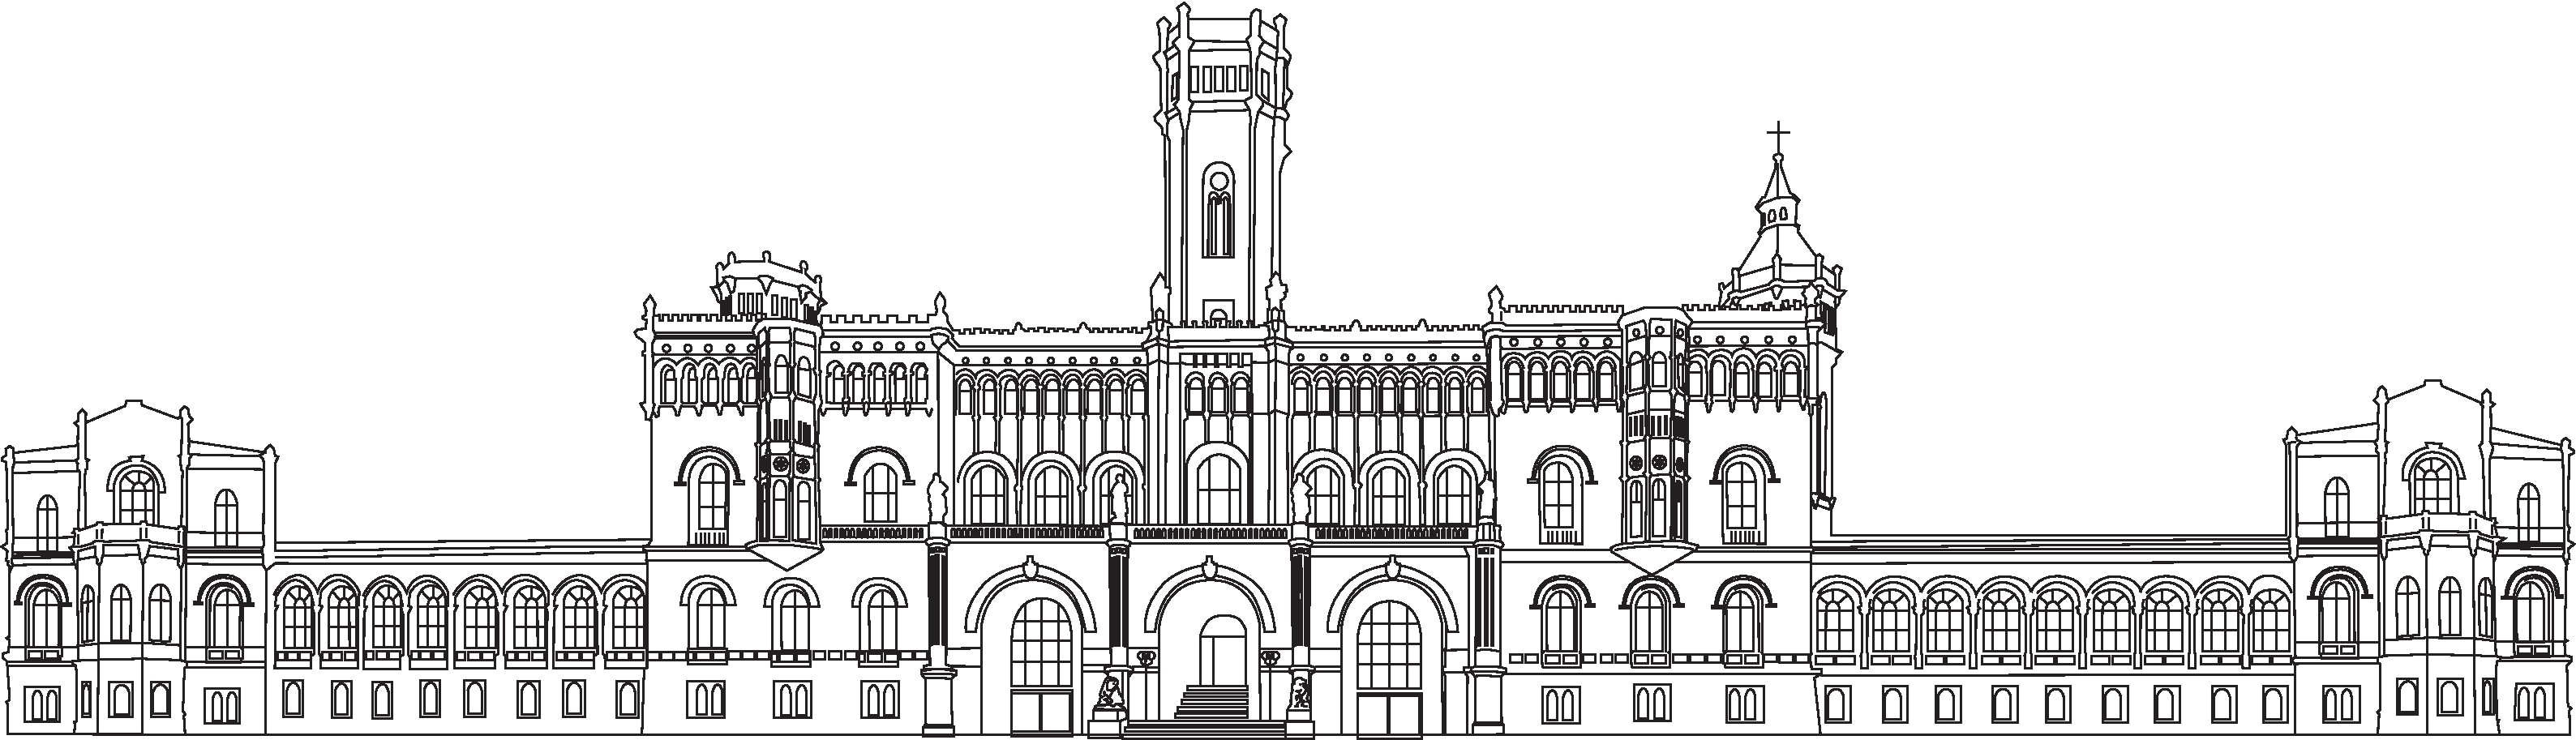
\includegraphics[width=13.8cm]{img/welfenschloss} \\
  \end{center}
  \medskip
  \begin{center}
    \textbf{\huge\spacedallcaps{L}\LARGE\spacedallcaps{eibniz}}
    \textbf{\huge\spacedallcaps{U}\LARGE\spacedallcaps{niversit\"{a}t}}
    \textbf{\huge\spacedallcaps{H}\LARGE\spacedallcaps{annover}} \\
  \end{center}

  \begin{center}
    \normalsize
    \spacedallcaps{Fakult\"{a}t}
    \spacedallcaps{f\"{u}r}
    \spacedallcaps{Elektrotechnik}
    \spacedallcaps{und}
    \spacedallcaps{Informatik} \\
    \smallskip
    \spacedallcaps{Institut}
    \spacedallcaps{f\"{u}r}
    \spacedallcaps{Praktische Informatik}
  \end{center}
  \vfill
  \vfill


  {
    %*******************************************************
    % Titlepage for everyone else 
    %*******************************************************
    \begin{center}
      \LARGE \myTitle{}
    \end{center}
    \vfill
    \vfill

    \begin{center}
      \LARGE \textbf{\myDegree}
    \end{center}
    \vfill

    \begin{center}
      \large submitted by \\
    \end{center}

    \begin{center}
      \large \spacedallcaps{\myName}
    \end{center}

    \begin{center}
      \large on \myTime{} \\
    \end{center}
    \vfill

    \begin{center}
      \begin{tabular}{lll}
        First Examiner  & : & \myProf{}       \\ % chktex 26
        Second Examiner & : & \myOtherProf{}  \\ % chktex 26
        Supervisor      & : & \mySupervisor{} % chktex 26
      \end{tabular}
    \end{center}

  }  % end condWIWI

  %  \vfill

  %  \begin{center}
  %    \large \selectedthesisnumber \\
  %  \end{center}

  \changetext{}{-21mm}{}{-19mm}{}

\end{titlepage}

\thispagestyle{empty}

\hfill

\vfill

\noindent\myName: \textit{\myTitle,}
%\mySubtitle,
%\myDegree,
\textcopyright{}~\myTime{}

%\bigskip
%
%\noindent\spacedlowsmallcaps{Supervisors}: \\
%\myProf \\
%\myOtherProf \\
%\mySupervisor
%
%\medskip
%
%\noindent\spacedlowsmallcaps{Location}: \\
%\myLocation
%
%\medskip
%
%\noindent\spacedlowsmallcaps{Time Frame}: \\
%\myTime

\cleardoublepage{}
%*******************************************************
% Declaration
%*******************************************************
\pdfbookmark[1]{Declaration}{declaration}
\chapter*{Declaration}
\thispagestyle{empty}
I hereby affirm that I have completed this work without the help of third parties and only with the sources and aids indicated. All passages that were taken from the sources, either verbatim or in terms of content, have been marked as such. This work has not yet been submitted to any examination authority in the same or a similar form.
\bigskip

\noindent\textit{\myLocation{}, \myTime{}}

\smallskip

\begin{flushright}
    \begin{tabular}{m{5cm}}
        \\ \hline % chktex 44
        \centering\myName{} \\
    \end{tabular}
\end{flushright}

% \cleardoublepage{}
% %*******************************************************
% Dedication
%*******************************************************
\thispagestyle{empty}
\phantomsection{}
\pdfbookmark[1]{Dedication}{Dedication}

\vspace*{3cm}

\begin{center}
    \emph{Ohana} means family. \\
    Family means nobody gets left behind, or forgotten. \\ \medskip
    --- Lilo \& Stitch
\end{center}

\medskip

\begin{center}
    Dedicated to the loving memory of Rudolf Miede. \\ \smallskip
    1939\,--\,2005
\end{center}

\cleardoublepage{}
%*******************************************************
% Abstract
%*******************************************************
%\renewcommand{\abstractname}{Abstract}
\pdfbookmark[1]{Abstract}{Abstract}
% \addcontentsline{toc}{chapter}{\tocEntry{Abstract}}
\begingroup
\let\clearpage\relax
\let\cleardoublepage\relax
\let\cleardoublepage\relax
%! TODO
\chapter*{Abstract}
The discovery of primary key candidates and unique columns in general is an important problem. % TODO: write better
The current algorithms to find unique columns are not fast enough for large tables as their runtime depends on the size of the table.

In this thesis, I propose a new method to detect unique columns. It uses a machine learning model to predict which columns are probably unique columns. Only positive guesses will be checked for duplicates. With this method, the time it takes to detect all unique columns is reduced by more than \SI{60}{\percent} for large tables with more than \num{10000000} rows. % TODO: is this number correct?

\endgroup


\cleardoublepage{}
% LTex: enabled=false
%*******************************************************
% Table of Contents
%*******************************************************
\pagestyle{scrheadings}
%\phantomsection
\pdfbookmark[1]{\contentsname}{tableofcontents}
\setcounter{tocdepth}{2} % <-- 2 includes up to subsections in the ToC
\setcounter{secnumdepth}{3} % <-- 3 numbers up to subsubsections
\manualmark{}
\markboth{\spacedlowsmallcaps{\contentsname}}{\spacedlowsmallcaps{\contentsname}}
\tableofcontents{}
\automark[section]{chapter}
\renewcommand{\chaptermark}[1]{\markboth{\spacedlowsmallcaps{#1}}{\spacedlowsmallcaps{#1}}}
\renewcommand{\sectionmark}[1]{\markright{\textsc{\thesection}\enspace\spacedlowsmallcaps{#1}}}
%*******************************************************
% List of Figures and of the Tables
%*******************************************************
\clearpage
% \pagestyle{empty} % Uncomment this line if your lists should not have any headlines with section name and page number
\begingroup
\let\clearpage\relax
\let\cleardoublepage\relax
%*******************************************************
% List of Figures
%*******************************************************
%\phantomsection
%\addcontentsline{toc}{chapter}{\listfigurename}
\pdfbookmark[1]{\listfigurename}{lof}
\listoffigures

\vspace{8ex}

%*******************************************************
% List of Tables
%*******************************************************
%\phantomsection
%\addcontentsline{toc}{chapter}{\listtablename}
\pdfbookmark[1]{\listtablename}{lot}
\listoftables

\vspace{8ex}
% \newpage

%*******************************************************
% List of Listings
%*******************************************************
%\phantomsection
%\addcontentsline{toc}{chapter}{\lstlistlistingname}
\pdfbookmark[1]{\lstlistlistingname}{lol}
\lstlistoflistings{}

\vspace{8ex}

%*******************************************************
% Acronyms
%*******************************************************
%\phantomsection
% \pdfbookmark[1]{Acronyms}{acronyms}
% \markboth{\spacedlowsmallcaps{Acronyms}}{\spacedlowsmallcaps{Acronyms}}
% \chapter*{Acronyms}
% \begin{acronym}[UMLX]
%     \acro{ai}[AI]{Artificial Intelligence}
%     \acro{auto-ml}[Auto-ML]{automated machine learning}
%     % \acro{acronym}[short name]{long name}
% \end{acronym}

\endgroup

%********************************************************************
% Mainmatter
%*******************************************************
\cleardoublepage{}
\pagestyle{scrheadings}
\pagenumbering{arabic}
% use \cleardoublepage here to avoid problems with pdfbookmark
\cleardoublepage{}

% \ctparttext{You can put some informational part preamble text here.
%     Illo principalmente su nos. Non message \emph{occidental} angloromanic
%     da. Debitas effortio simplificate sia se, auxiliar summarios da que,
%     se avantiate publicationes via. Pan in terra summarios, capital
%     interlingua se que. Al via multo esser specimen, campo responder que
%     da. Le usate medical addresses pro, europa origine sanctificate nos se.}
% \cleardoublepage{}

\section{Basics}
\begin{itemize}
  \item Introduce the subjects used in the thesis
  \item The explanations have to be sufficient for a student after the lecture DBS~I
\end{itemize}

\subsection{Dataset}
\begin{itemize}
  \item Give an overview over the dataset(s) used in the thesis
  \item Probably short, the points are
        \begin{itemize}
          \item[(!)] Structure of the dataset in the database and the way it gets converted
          \item[(!)] Size of the dataset
          \item[(?)] Possible contents or their form
          \item[(?)] Where the data came from
        \end{itemize}
  \item This could be its \underline{own chapter}.
\end{itemize}
\section{Machine Learning}\label{sec:machine_learning}
Machine learning is a part of the field of \ac{ai}. The focus is on extracting information from large amounts of data, with algorithms gradually improving themselves to mimic human learning~\cite{what-is-ml}.

The field of machine learning is itself divided into two main parts, Classical learning and Deep learning\cite{ml-visual-explanation}.

% https://ischoolonline.berkeley.edu/blog/what-is-machine-learning/
% https://www.ibm.com/cloud/learn/machine-learning

\subsection{Deep Learning and Neural Networks} % TODO: need to proof read

Deep Learning includes various techniques that use neural networks. In the simplest form, neural networks consist of different so-called nodes, which are arranged as layers\cite{neuralNet}.

The first layer, also known as the \enquote{input layer}, is the layer the input vector is applied to. If the input exceeds a certain value, the neuron is activated, i.e.\ it passes on an output.

In the next layers, which are called \enquote{hidden layers}, the outputs from all the nodes of the previous layer and a \enquote{bias layer} are computed in each node and the output is passed on. The bias layer consists of a single value that influences all nodes on a layer.

Finally, the last layer outputs the result of the computation. How strong each previous node influences the value of the current node is what the neural network is trained on.

Neural networks are particularly good at recognizing patterns in large unordered data, such as images, videos, and audio tracks. Examples of this include facial recognition or verifying hand signatures\cite{neuralNet-applications}.

\newcommand{\neuralx}[2]{\(x_#2\)}
\newcommand{\neuraly}[2]{\(\hat{y}_#2\)}
\newcommand{\neuralh}[2]{\small \(h^{(#1)}_#2\)}
\begin{figure}[ht]
  \centering
  \caption[An example of a neural network]{A simple neural network with three input nodes and two output nodes.}
  \begin{neuralnetwork}[height=5]
    \inputlayer[count=3, bias=false, title=Input\\layer, text=\neuralx]
    \hiddenlayer[count=4, bias=true, title=Hidden\\layer 1, text=\neuralh] \linklayers{}
    \hiddenlayer[count=3, bias=false, title=Hidden\\layer 2, text=\neuralh] \linklayers{}
    \outputlayer[count=2, title=Output\\layer, text=\neuraly] \linklayers{}
  \end{neuralnetwork}\label{fig:neural_network}
\end{figure}

\subsection{Classical Learning} % TODO: writing
% https://towardsdatascience.com/deep-learning-vs-classical-machine-learning-9a42c6d48aa
Algorithms in the field of classical machine learning are largely based on statistical or probabilistic methods, which originated as pattern recognition in the 1960s. It has the advantage of being a fast method that does not require much computing power compared to deep learning algorithms\cite{classical-ml}.

%! TODO: another paragraph

\subsection{Categories of Machine Learning}
Both deep learning as well as classical learning are dived into different categories which are based on the kind of task and trainingsdata the machine learning models have to work with.

Unsupervised learning is used on unlabeled data. Its main use is to organize the data or to make it more manageable. Tasks in this domain include clustering, which categorizes data based on similar data points, or assoziation, which tries to find relationships between variables in a dataset\cite{supervised-unsupervised-learning}.

Supervised learning on the other hand makes use of labeled data. This comes with the disadvantage that the structure of the data as well as the desired results have to be known\cite{classical-ml}. Even though it increases the effort of the preparation of the trainingsdata, it also raises the accuracy of the model since it is trained to produce exactly the desired result.

% TODO: what and why labeled data?

% Reinforcement Learning  \cite{types-of-ml} %! TODO

\begin{figure}[ht]
  \caption[Different kinds of machine learning]{This picture shows the different types of machine learning and the way they are trained\cite{types-of-ml}.} % TODO: is a more detailed description necessary?
  \centering
  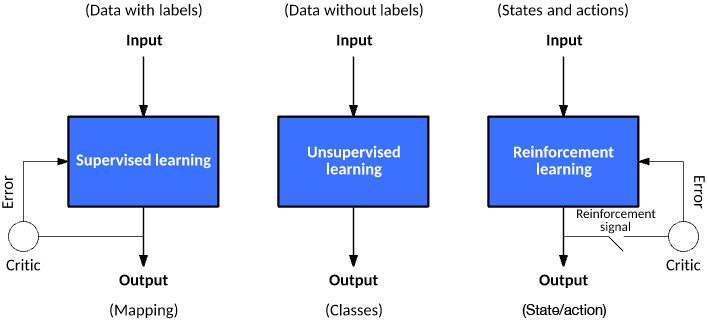
\includegraphics[width=\linewidth]{img/types_of_machine_learning.png}\label{fig:kinds_of_ml}
\end{figure}

\section{Existing Algorithms}

\section{Naive Algorithms}
\begin{itemize}
  \item This will be very short as the basic way of finding unique columns is known by the target group
  \item If the naive algorithms are implemented with flipped tables, explain it here
\end{itemize}

\subsection{Related Work}
\begin{itemize}
  \item Maybe here, maybe at the end
  \item Possibly a small comparison here and a longer one in its own section
\end{itemize}


% ********************************************************************
% Backmatter
%*******************************************************
\appendix
%\renewcommand{\thechapter}{\alph{chapter}}
\cleardoublepage{}
% \part{Appendix}

%********************************************************************
% Other Stuff in the Back
%*******************************************************
\cleardoublepage{}
%********************************************************************
% Bibliography
%*******************************************************
% work-around to have small caps also here in the headline
% https://tex.stackexchange.com/questions/188126/wrong-header-in-bibliography-classicthesis
% Thanks to Enrico Gregorio
\defbibheading{bibintoc}[\bibname]{%
  \phantomsection{}
  \manualmark{}
  \markboth{\spacedlowsmallcaps{#1}}{\spacedlowsmallcaps{#1}}%
  \addtocontents{toc}{\protect\vspace{\beforebibskip}}%
  \addcontentsline{toc}{chapter}{\tocEntry{#1}}%
  \chapter*{#1}%
}
\printbibliography[heading=bibintoc]

% Old version, will be removed later
% work-around to have small caps also here in the headline
%\manualmark
%\markboth{\spacedlowsmallcaps{\bibname}}{\spacedlowsmallcaps{\bibname}} % work-around to have small caps also
%\phantomsection
%\refstepcounter{dummy}
%\addtocontents{toc}{\protect\vspace{\beforebibskip}} % to have the bib a bit from the rest in the toc
%\addcontentsline{toc}{chapter}{\tocEntry{\bibname}}
%\label{app:bibliography}
%\printbibliography

% ********************************************************************
% Game Over: Restore, Restart, or Quit?
%*******************************************************
\end{document}
% ********************************************************************
